\documentclass[./project-report/src/latex/project-report.tex]{subfiles}

\begin{document}

\maketitle

\section{Technical Solution TODO}

\subsection{Setup}

\subsubsection{File Structure}

I used the following file structure to organise the code for the project, where school\_project is the package and is constructed of two main modules:

\begin{itemize}
    \item The models module, which is a self-contained module for creating trained Artificial Neural Network models.
    \item The frames module, which consists of tkinter frames for the User Interface.
\end{itemize}

Each module within the school\_project package contains a \_\_init\_\_.py file, which allows the package to be installed to a virtual environment so that the modules of the package 
can be imported from the installed package. I have omitted the source code for this report, which included a Makefile for its compilation.

\pagebreak

\begin{footnotesize}
\verbatiminput{|"git ls-tree -r --name-only HEAD | grep -v -E 'project-report/|Makefile' | tree --fromfile --charset=ascii"}  % TODO: Could include project-report and Makefile
\end{footnotesize}

\subsubsection{Dependencies}

The python dependencies for the project can be installed simply by running the following setup.py file (as described in the README.md in the next section). Instructions on 
installing external dependencies, such as the CUDA Toolkit for using a GPU, are explained in the README.md in the next section also.

\begin{itemize}
    \item setup.py code:
        \inputminted{python}{./setup.py}
\end{itemize}

\subsubsection{Git and Github files}

To optimise the use of Git and GitHub, I have used the following files:

\begin{itemize}
    \item A .gitignore file for specifying which files and directories should be ignored by Git:
        \inputminted{text}{./.gitignore}
    \item A README.md markdown file to give installation and usage instructions for the repository on GitHub:
        \begin{itemize}
            \item Markdown code:
                \inputminted{markdown}{./README.md}
            \item Which will generate the following:
                \pagebreak
                \begin{figure}[h!]
                \centering
                
\includegraphics[width=1\textwidth]{./project-report/src/images/readme-top.png}
                \end{figure}
                \pagebreak
                \begin{figure}[h!]
                \centering
                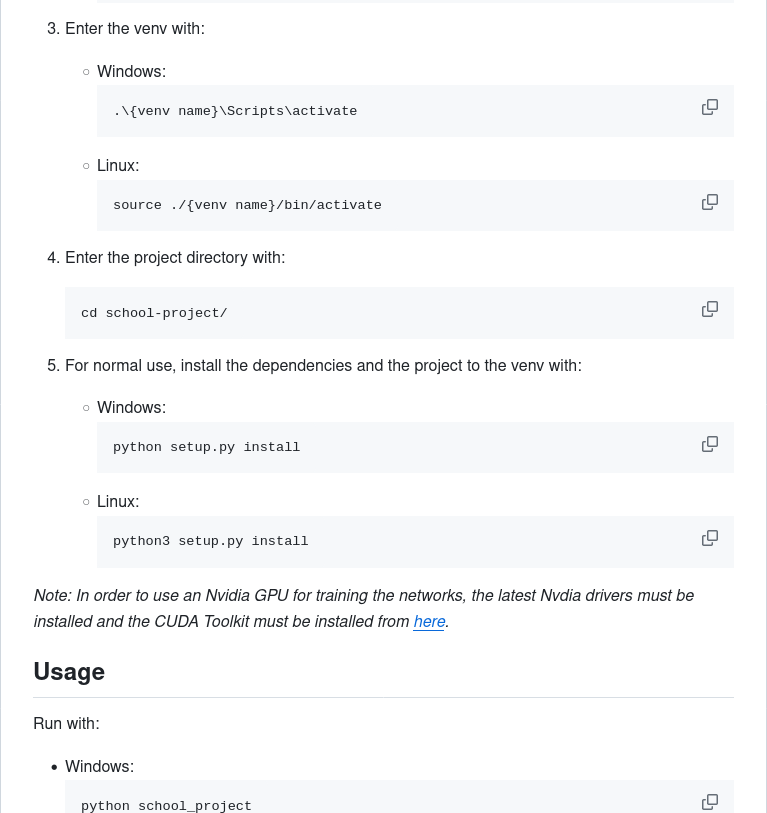
\includegraphics[width=1\textwidth]{./project-report/src/images/readme-middle.png}
                \end{figure}
                \pagebreak
                \begin{figure}[h!]
                \centering
                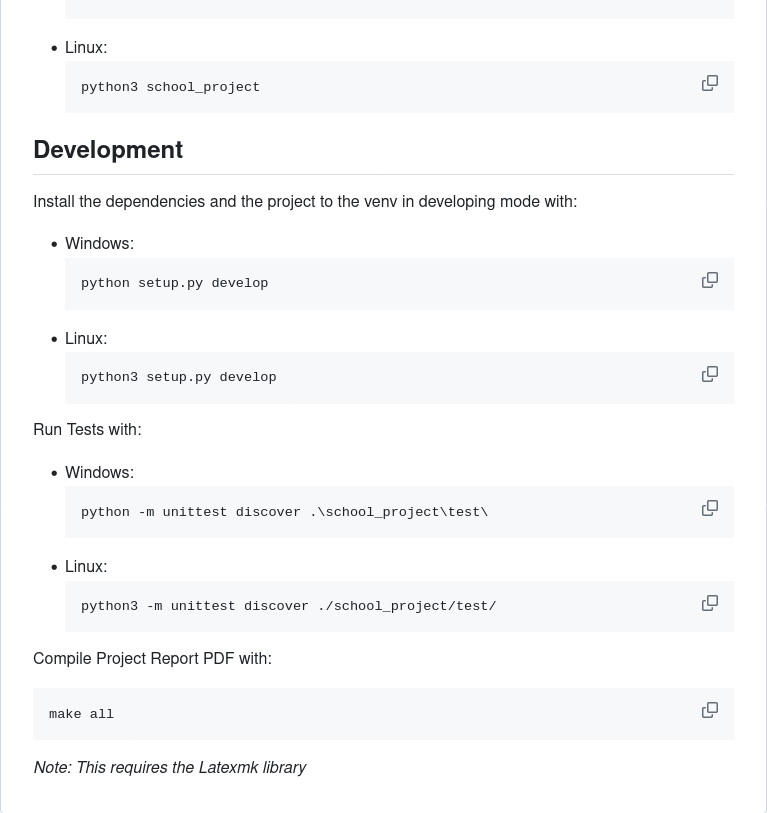
\includegraphics[width=1\textwidth]{./project-report/src/images/readme-bottom.png}
                \end{figure}
        \end{itemize}
    \item A LICENSE file that describes how others can use my code.
\end{itemize}

\subsubsection{Organisation}

I also utilise a TODO.md file for keeping track of what features and/or bugs need to be worked on.

\end{document}